\section{Finite Differences Method for Parabolic PDEs}

\subsection{Richardson's \emph{Explicit} FD Scheme}

\begin{enumerate}
	\item \emph{Discretise parabolic PDE} $Lu(...) = f(...)$ using discrete operators
	\item{
		\emph{Discretise geometry} by introducing a grid:
		$x_{j,k} = (j\cdot\Delta x, k\cdot\Delta t)$ with $j$ as the local index
		and $k$ as the time index where $k=0$ is on boundary
		and \colorbox{shadecolor}{$\Delta x = \frac{1}{n}$},
		\colorbox{shadecolor}{$\Delta t = \frac{r}{n^2}$}
		and \colorbox{shadecolor}{$r = \frac{\Delta t}{\Delta x^2}$}
	}
	\item{
		\emph{Introduce approximated nodal values} $\utild(x_{j,k}) = \utild_{j,k}$ and $f_j = f(x_j,0)$ for the Dirichlet boundary conditions.
	}
	\item{
		Find a matrix $C$ that satisfies

		\colorbox{shadecolor}{$
			\displaystyle
			\utild_{j}^{(k+1)}=r\utild_{j-1}^{(k)}+(1-2r)\utild_{j}^{(k)} + r\cdot \utild_{j+1}^{(k)}
		$}

		for inner grid points for each ``step`` satisfying boundary conditions: $\utild_{j}^{(0)}=\utild_{j,0}=f_j$
	}
	\item{
		Iteratively generate solution vector using $\utild^{(k+1)}=C\cdot\utild^{(k)}$
		(i.e. $\utild^{(k)} = C^k\cdot \vec{f}$)
	}
\end{enumerate}

\subsubsection{Stability Analysis}

\begin{wrapfigure}{r}{0.25\columnwidth}
	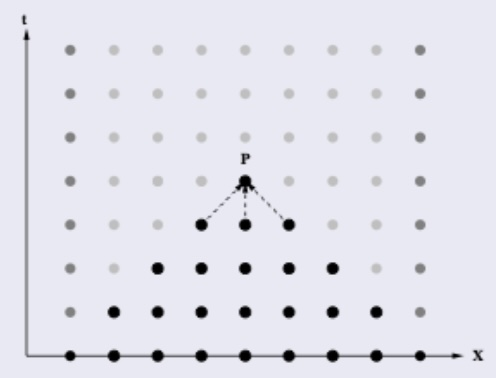
\includegraphics[width=0.25\columnwidth]{images/richardsons}
\end{wrapfigure}

The scheme of Richardson tends asymptotically to zero with k to infinity if
for eigenvalues of $C$, $|\lambda_\mathrm{max}|<1$ is true or $||C^{(n)}||<1$ with respect to the spectral norm of C.

We only receive a good approximation if the steps are small enough to ``catch'' enough information on the boundary.

\subsubsection{Example Using Heat Equation}

\textbf{Given} the heat equation $\frac{\partial u}{\partial t}(x,t) = \frac{\partial^2 u}{\partial x^2}(x,t)$
for the domain $\Omega = [0,1]\times [0, \infty[$ with the boundary conditions
$u(x,0) = e^x$, $u(0,t) = e^t$ and $u(1,t) = e^{1+t}$, we want to find an approximation $\utild$ for points
$(1/3,2/3),(2/3,2/3)$ using $\Delta x = 1/3$ and $\Delta t = 1/3$.

\textbf{Discretisation of Heat Equation}:
\begin{align*}
	& \frac{u(x,t+\Delta t)-{\color{blue} u(x,t)}}{\color{blue}\Delta t}\approx\frac{u(x+\Delta x,t)-2\cdot u(x,t)+u(x-\Delta x,t)}{\Delta x^{2}} \\
	& u(x,t+\Delta t)\approx {\color{blue}u(x,t)+\Delta t}\cdot{\frac{u(x+\Delta x,t)-2 u(x,t)+u(x-\Delta x,t)}{\Delta x^{2}}} \\
	& \utild_{j,k+1}=u_{j,k}+r\cdot u_{j+1,k} - 2u_{j,k} + u_{j-1,k}\quad \left|r=\frac{\Delta t}{\Delta x^2}\right. \\
	& \utild_{j,k+1} = r\cdot\utild_{j-1,k}+(1-2r)\utild_{j,k} + r\cdot\utild_{j+1,k}
\end{align*}

\textbf{Discretisation of Geometry}:

\makebox[\columnwidth]{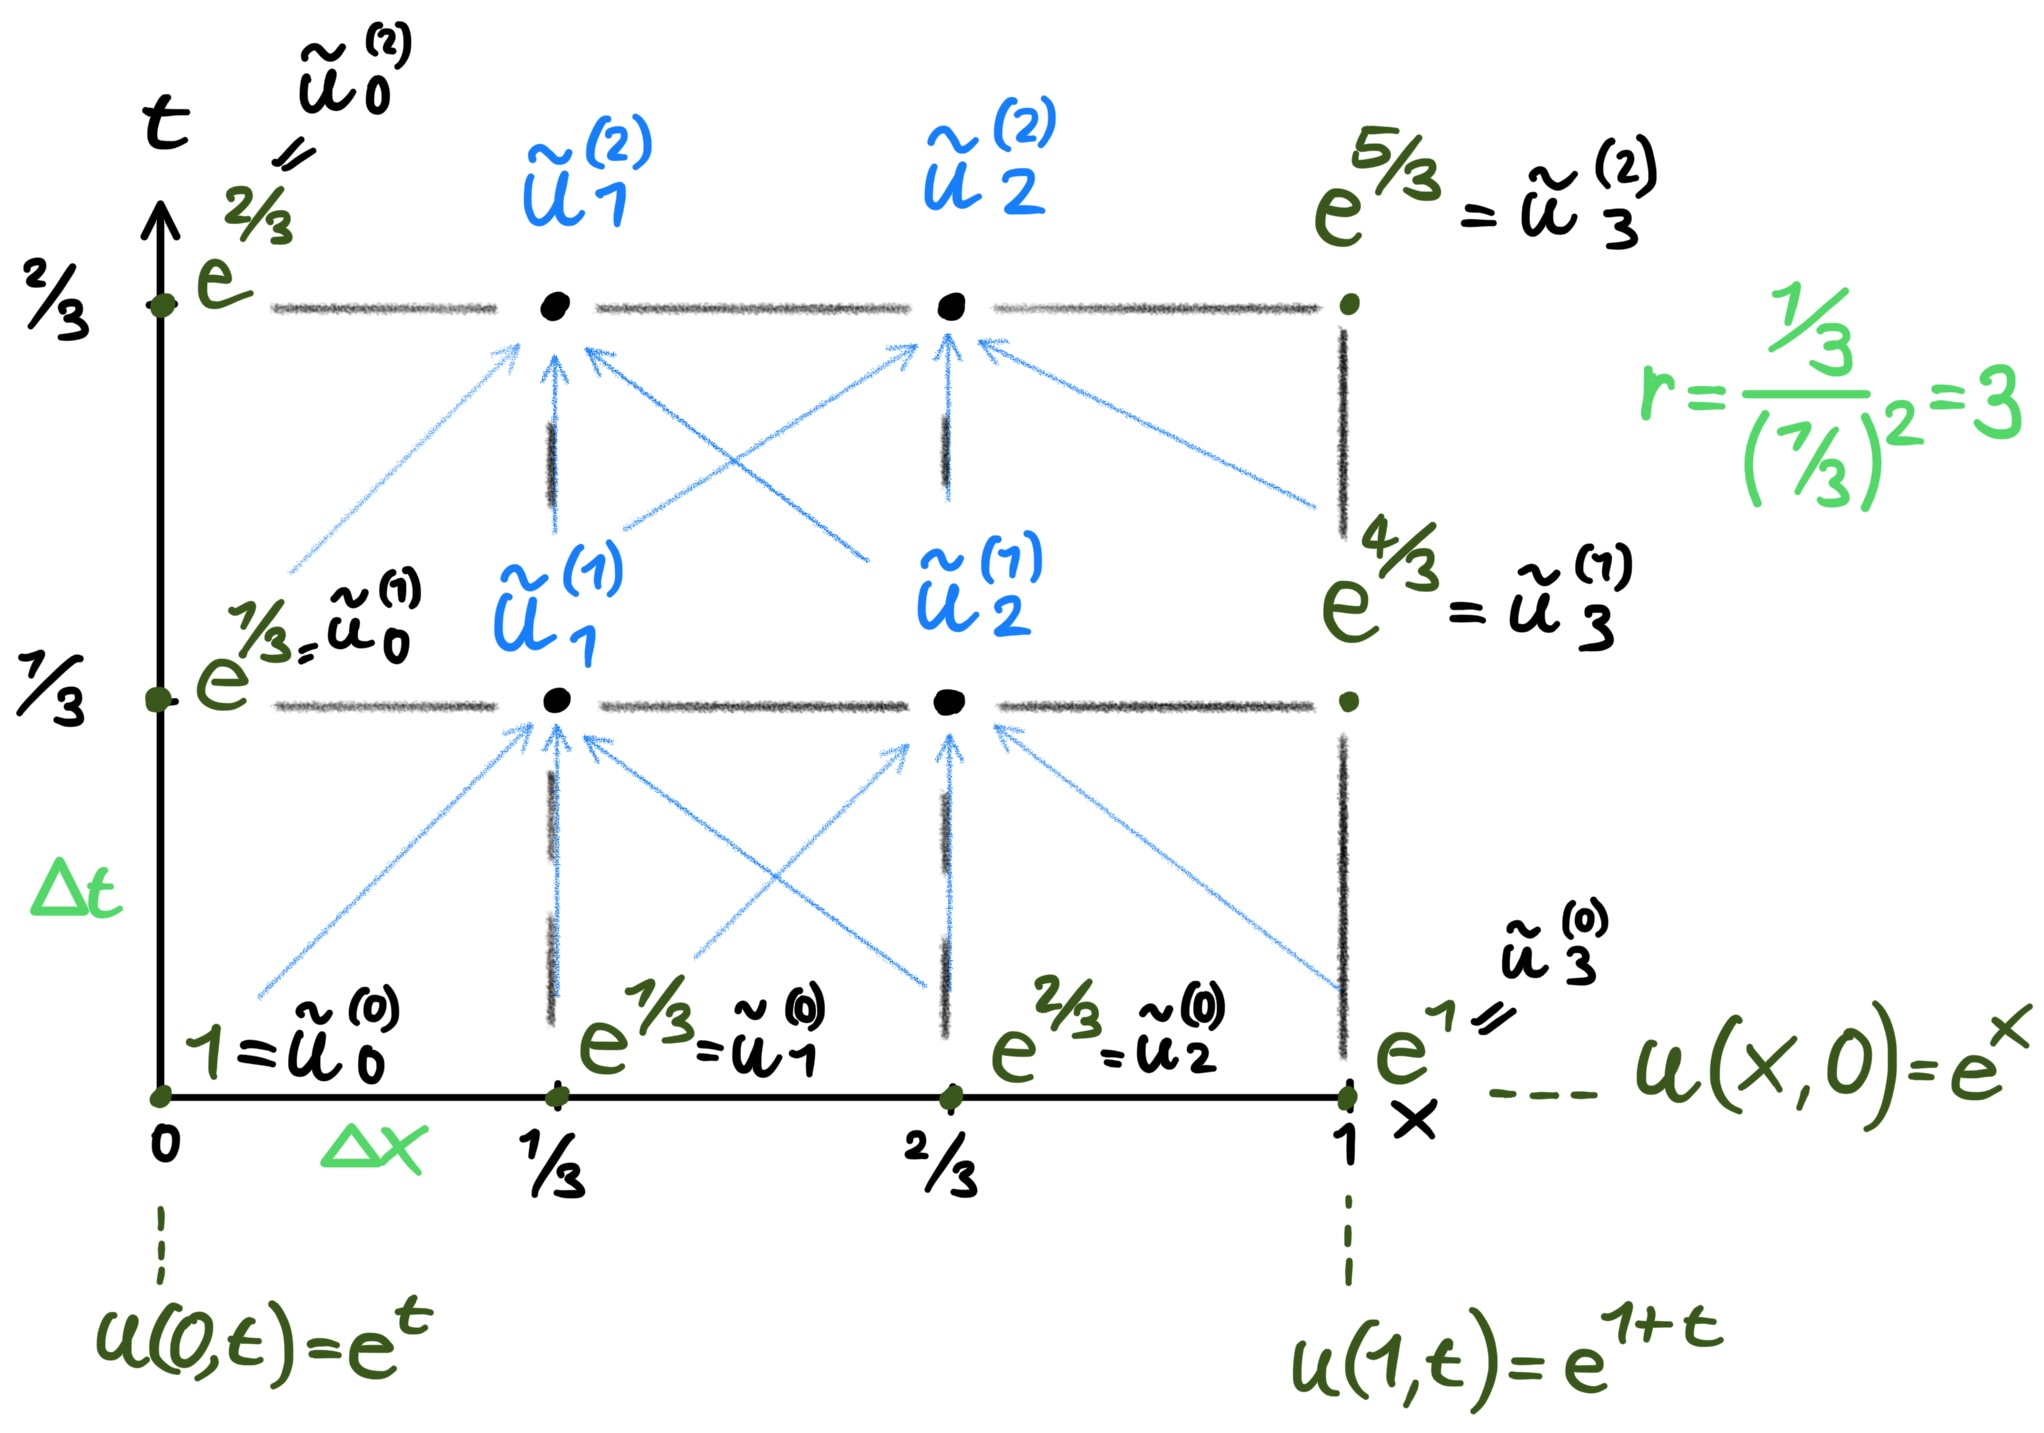
\includegraphics[width=0.75\columnwidth]{images/richardson_explicit}}

\textbf{Solution Method:} With $r$ having a set value, we can write the iterative equation as:
\begin{align*}
	\utild_{j}^{(k+1)} = 3\utild_{j-1}^{(k)} + 5\utild_{j}^{(k)} + 3\utild_{j+1}^{(k)}
\end{align*}

and thus, for $\mathbf{k+1=1}$:
\begin{align*}
	\utild_1^{(1)} & = 3\cancelto{1}{\utild_0^{(0)}} - 5\cancelto{e^{1/3}}{\utild_1^{(0)}} + 3\cancelto{e^{2/3}}{\utild_2^{(0)}} {\color{gray} = 1.8651} \\
	\utild_2^{(1)} & = 3\utild_1^{(0)} - 5\utild_2^{(0)} + 3\utild_3^{(0)} {\color{gray} = 2.603}
\end{align*}

and $\mathbf{k+1 = 2}$:
\begin{align*}
	\utild_1^{(2)} & = 3\cancelto{e^{\Delta t\cdot k}}{\utild_0^{(1)}} - 5\utild_1^{(1)} + 3\utild_2^{(1)} {\color{gray} = 2.6702} \\
	\utild_2^{(2)} & = 3\utild_1^{(1)} - 5\utild_2^{(1)} + 3\cancelto{e^{1+\Delta t\cdot k}}{\utild_3^{(1)}} {\color{gray} = 3.9614}
\end{align*}

Alternatively, using matrix $C$:
\begin{align*}
	\begin{bmatrix}
		\utild_1 \\
		\utild_2
	\end{bmatrix}^{(k+1)}
	=
	\underbrace{
		\begin{bmatrix}
			-5 & 3 \\
			3 & -5
		\end{bmatrix}
	}_{C}
	\begin{bmatrix}
		\utild_1 \\
		\utild_2
	\end{bmatrix}^{(k)}
	+
	\underbrace{
		3\begin{bmatrix}
			e^{\Delta t k} = e^\frac{k}{3} \\
			e^{1+\Delta t k} = e^{1+\frac{k}{3}}
		\end{bmatrix}
	}_\text{Dirichlet B.C.}
\end{align*}

and
\begin{align*}
	\begin{bmatrix}
		\utild_1 \\
		\utild_2
	\end{bmatrix}^{(2)}
	=
	C^2\vec{\utild}^{(0)} + C\cdot 3\begin{bmatrix}
		1 \\
		e
	\end{bmatrix}
	+
	3\begin{bmatrix}
		e^{1/3} \\
		e^{4/3}
	\end{bmatrix}
	{\color{gray}
		=
		\begin{bmatrix}
			2.6702 \\
			3.9614
		\end{bmatrix}
	}
\end{align*}
